\documentclass{cilamce19}

\begin{document}
%Insert the header


%%This is the short title that will be inside the header 
\shorttitle{Put your short title in here.}
 
\begin{titlepage}
	
	\newgeometry{top=1.3in,bottom=0.8in,right=0in,left=2in}

	
	\begin{figure}
	\flushright
	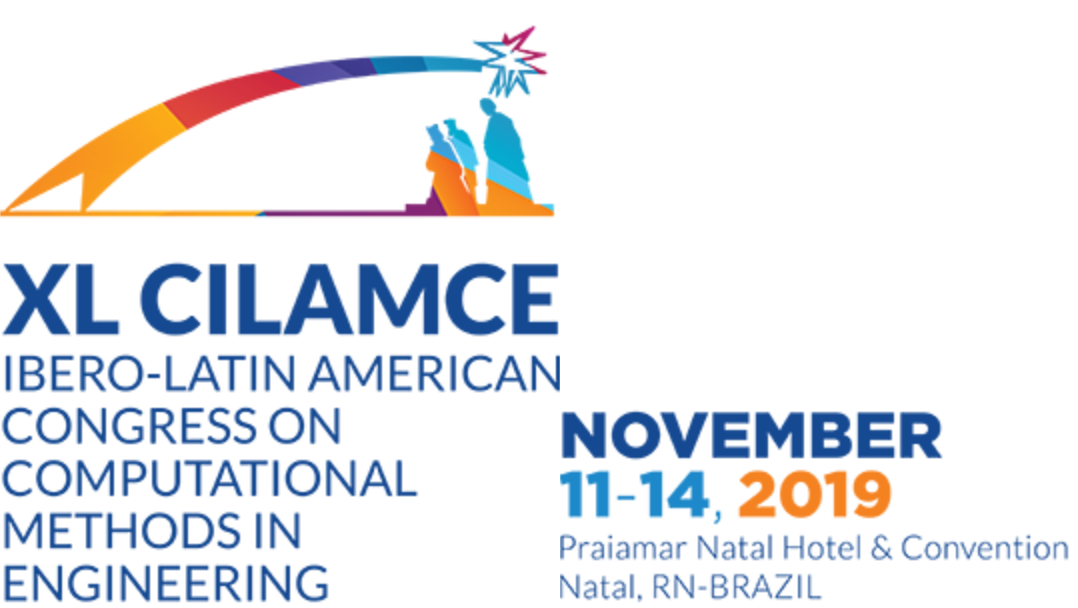
\includegraphics[width=1.66in]{clm19.png}
    \end{figure}


 \begin{center}
 	\begin{title}
 		\centering
 		\textbf{INSTRUCTIONS FOR PREPARATION AND SUBMISSION OF FULL-PAPERS FOR PUBLICATION IN THE PROCEEDINGS OF XL CILAMCE AND STARTS CILAMCE19.CLS V1.01}
 	\end{title}	
 \end{center}



%Authors and Affiliations
\textbf{First A. Author}
\\
\textbf{Second B. Author}
\\
\textit{somebody1@somewhere.com}\\
\textit{somebody2@somewhere.com}
\\
\textbf{Affiliation}
\\
\textit{Address, Zip-Code, State/Province, Country}
\\
\textbf{Third C. Author}
\\
\textit{somebody3@elsewhere.com}\\
\textbf{Affiliation}
\\
\textit{Address, Zip-Code, State/Province, Country}
\\

%Abstract
\textbf{Abstract:}This document-template provides detailed instructions for preparing and submitting a paper to the XL Ibero-Latin American Congress on Computational Methods in Engineering (CILAMCE-2019). Please follow these general instructions carefully: (a) type the body of the paper in single column; (b) use no more than 20 A4-size pages (maximum 5 pages for papers at the Research Beginners Mini-symposium), each formatted with 2.5 cm margins on all sides (do not insert page numbers); (c) use 11pt Times New Roman throughout the body of the text, with 13 pt for the title andfirst-level headings (we strongly encourage you to use the pre-defined styles of this template, as they embed all necessary text formatting for the corresponding paragraph type); (d) type up to 250 words in the abstract; (e) always use either single-spaced orexactly 13-pt-spaced lines, with justified alignment; (f) cite references by Name [number],and list them consecutively in the reference list by the order of citationin the text (the list should only include works that are cited in the text); (g) provide good quality figures; (h) define all quantities, variables and symbols as soon as they first appear in the text; (i) equations must be typed either in Math type or MS Equation (or similar); (j) use only SI units. It is strongly recommended that the paper be written in English. Papers in Portuguese, Spanish or Italian may be occasionally accepted, provided that at least the abstract and the slides for oral presentation are in English

%Keywords
\textbf{Keywords:} Cilamce, Ibero-Latin, MS Equation.
\end{titlepage}




%Here your work really starts.
\section{Introduction}
   \lipsum[1]
   \citet{book-example}


\section{Methodology}

 \lipsum[2-4]\citet{article-example}


\section{Results}
\lipsum[6-7]\citet{inbook-example}

\section{Conclusions}
\lipsum[8-11]

\section{Acknowledgements}
\lipsum[12]

%\bibliographystyle{abbrv}
  \bibliography{references.bib}
  
\end{document} 
